\documentclass[11pt,a4paper]{report}

\usepackage[utf8]{inputenc}
\usepackage[T1]{fontenc}\usepackage[spanish]{babel}
\usepackage[notes,backend=biber]{biblatex-chicago}

\usepackage{graphicx}
\graphicspath{ {./imagenes/} }

\usepackage{listings}
\usepackage{float}
\usepackage{csquotes}


\lstset{
	  frame=tb,
	  language=Java,
	  aboveskip=3mm,
	  belowskip=3mm,
	  showstringspaces=false,
	  columns=flexible,
	  basicstyle={\small\ttfamily},
	  numbers=none,
	  breaklines=false,
	  breakatwhitespace=true,
	  tabsize=1
}

\begin{document}
	\begin{titlepage}
		\centering
		{\scshape\huge\bfseries INSTITUTO POLITÉCNICO NACIONAL \par}
		\vspace{0.7cm}
		{\scshape\LARGE\bfseries Escuela Superior de Computo \par}
		\vspace{0.5cm}
		{\scshape\Large \par}
		\vspace{1.5cm}
		{\Large\bfseries Reporte: \par}
		{\huge\bfseries Automatas \par}
		\vspace{2cm}
		{\LARGE\itshape Teoría Computacional\par}
		\vspace{0.2cm}
		{\Large Luis Diego Jimenez Delgado\par}
		\vfill
			{\scshape\Large 2CM5 \par}
			\vspace{0.5cm}
			{\scshape\large Profesor: \par}
			{\scshape\Large Genaro Juarez Martinez \par}
		\vfill
		{\large \today}
	\end{titlepage}
 
	\tableofcontents{}
	\chapter{Introducción}
Un autómata de pila es un modelo matemático de un sistema que recibe una cadena constituida por símbolos de un alfabeto y determina si esa cadena pertenece al lenguaje que el autómata reconoce.
Los autómatas de pila pueden aceptar lenguajes que no pueden aceptar los autómatas finitos. Un autómata de pila cuenta con una cinta de entrada y un mecanismo de control que puede encontrarse en uno de entre un número finito de estados. Uno de estos estados se designa como estado inicial, y además algunos estados se llaman de aceptación o finales. A diferencia de los autómatas finitos, los autómatas de pila cuentan con una memoria auxiliar llamada pila. Los símbolos (llamados símbolos de pila) pueden ser insertados o extraídos de la pila, de acuerdo con el manejo last-in-first-out (LIFO).
Las transiciones entre los estados que ejecutan los autómatas de pila dependen de los símbolos de entrada y de los símbolos de la pila. El autómata acepta una cadena x si la secuencia de transiciones, comenzando en estado inicial y con pila vacía, conduce a un estado final, después de leer toda la cadena x.
	\chapter{Autómata de cadena con terminación 01}
		\section{Programa}
\begin{lstlisting}
#include <stdio.h>
#include <stdlib.h>
#include "TADPilaDin.h"

/*
Cadena 0000000000011111111111
Compile: gcc app.c TADPilaDin.c -o a.out
*/

FILE *fp;
FILE *fanswer;
FILE *fstates;

void generateString(char *, int);
boolean isValidProcess();
char getChar();
void printStack(stack *from);

int main(int argc, const char **argv)
{
    char *file_name = "./prime.txt";
    if (argc == 2)
    {
        int n = atoi(argv[1]);
        generateString(file_name, n);
    }
    fp = fopen(file_name, "r");
    fstates = fopen("states.txt", "w");
    fanswer = fopen("answer.txt", "w");
    if (isValidProcess())
    {
        printf("Cadena valida\n");
    }
    else
    {
        printf("Cadena no valida\n");
    }
    fclose(fanswer);
    fclose(fstates);
    fclose(fp);
    return 0;
}

boolean isValidProcess()
{
    stack container;
    Initialize(&container);
    char toWork = getChar();
    element e;
    while (toWork != EOF)
    {
        while (toWork == '0')
        {
            e.c = 'x';
            Push(&container, e);
            printStack(&container);
            toWork = getChar();
        }
        while (toWork == '1')
        {
            if (!Empty(&container))
            {
                Pop(&container);
                printStack(&container);
                toWork = getChar();
            }
            else
            {
                Destroy(&container);
                return FALSE;
            }
        }
        toWork = getChar();
    }
    if (Empty(&container))
    {
        Destroy(&container);
        return TRUE;
    }
    else
    {
        Destroy(&container);
        return FALSE;
    }
}

char getChar()
{
    return (char)fgetc(fp);
}

void generateString(char *fileName, int number)
{
    FILE *generate;
    generate = fopen(fileName, "w");
    int i;
    printf("Generado cadena\n");
    if (number % 2 == 1)
        ++number;
    for (i = 0; i < (number / 2); ++i)
    {
        fputc('0', generate);
    }
    if (number % 2 == 1)
        ++number;
    for (i = 0; i < (number / 2); ++i)
    {
        fputc('1', generate);
    }
    fputc('\n', generate);
    fclose(generate);
}

void printStack(stack *from)
{
    stack helper1, helper2;
    Initialize(&helper1);
    Initialize(&helper2);
    printf("\nPila\n");
    while (!Empty(from))
    {
        element el;
        el = Pop(from);
        printf("-------\n");
        printf("---%c---\n", el.c);
        printf("-------\n");
        Push(&helper1, el);
    }
    printf("-------\n\n");
    while (!Empty(&helper1))
    {
        Push(&helper2, Pop(&helper1));
    }
    while (!Empty(&helper2))
    {
        element el;
        el = Pop(&helper2);
        Push(from, el);
    }
    Destroy(&helper1);
    Destroy(&helper2);
}
\end{lstlisting}
			\subsection{Input}
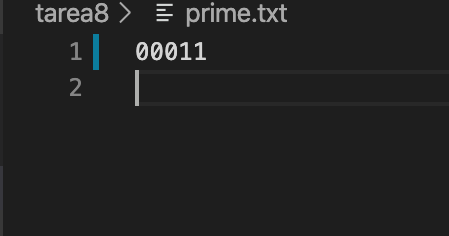
\includegraphics[scale=1.0]{tarea8i}\
			\subsection{Output}
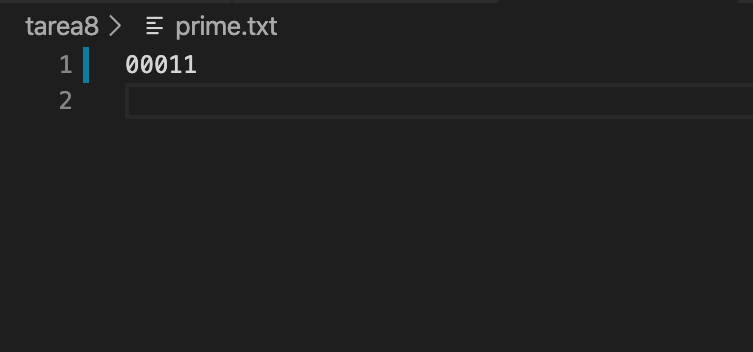
\includegraphics[scale=1.0]{tarea8o}\
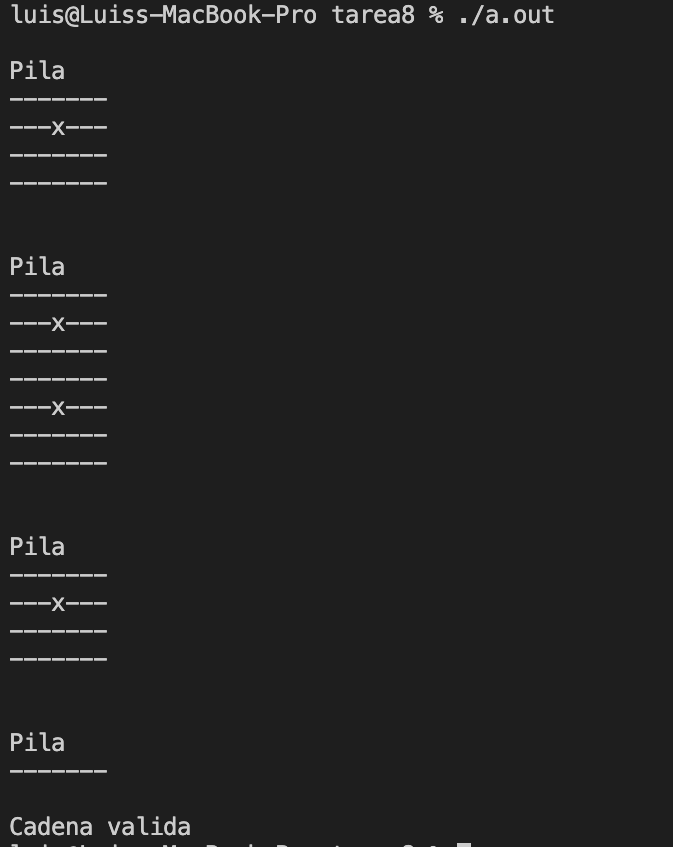
\includegraphics[scale=1.0]{tarea8o1}\

	\chapter{Cadena palindroma}
		\section{Programa}
\begin{lstlisting}
#include <stdio.h>
#include <stdlib.h>
#include "TADPilaDin.h"

/*
Cadena palindroma
Compile: gcc app.c TADPilaDin.c -o a.out
*/

char getChar();
void getString();
int getRandomNumber(int number);
int selectType();
int getBool();
void manageProcess();

FILE *fanswer;
FILE *fstates;
int length;

int main(int argc, const char **argv)
{
    int n = 100;
    arc4random();
    if (argc == 2)
    {
        n = atoi(argv[1]);
    }
    length = getRandomNumber(n);
    fanswer = fopen("./answer.txt", "w");
    manageProcess();
    fclose(fanswer);
    return 0;
}
void manageProcess()
{
    stack pila;
    Initialize(&pila);
    int type = selectType();
    element e;
    if (type == 1)
    {
        length = length - 2;
    }
    else
    {
        if (type == 2)
        {
            length = length - 2;
        }
        else
        {
            if (type == 3)
            {
                length = length - 1;
            }
            else
            {
                length = length - 1;
            }
        }
    }
    while (length >= 0)
    {
        if (getBool())
        {
            e.c = '0';
            Push(&pila, e);
            fputc('0', fanswer);
        }
        else
        {
            if (getBool())
            {
                e.c = '1';
                Push(&pila, e);
                fputc('1', fanswer);
            }
        }
        --length;
    }
    if (type == 1)
    {
        e.c = '0';
        Push(&pila, e);
        e.c = 'S';
        Push(&pila, e);
    }
    else
    {
        if (type == 2)
        {
            e.c = '1';
            Push(&pila, e);
            e.c = 'S';
            Push(&pila, e);
        }
        else
        {
            if (type == 3)
            {
                e.c = '0';
                Push(&pila, e);
            }
            else
            {
                e.c = '0';
                Push(&pila, e);
            }
        }
    }
    while (!Empty(&pila))
    {
        e = Pop(&pila);
        fputc(e.c, fanswer);
    }
    Destroy(&pila);
}
int selectType()
{
    return getRandomNumber(5);
}

int getBool()
{
    return getRandomNumber(2);
}

int getRandomNumber(int number)
{
    int res = rand();
    if (number > 0)
        res = rand() % number;
    return res;
}
\end{lstlisting}
			\subsection{Input}
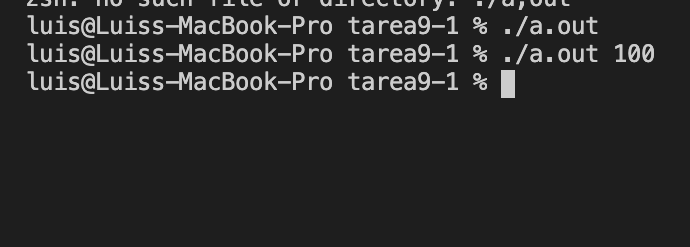
\includegraphics[scale=1.0]{tarea9i}\
			\subsection{Output}
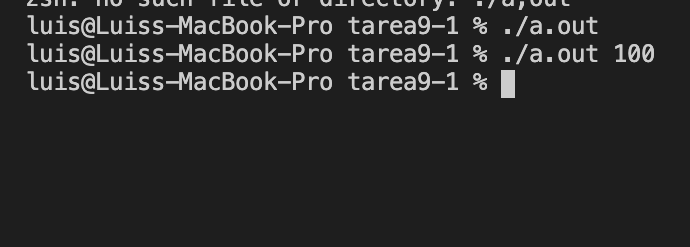
\includegraphics[scale=.80]{tarea9o}\
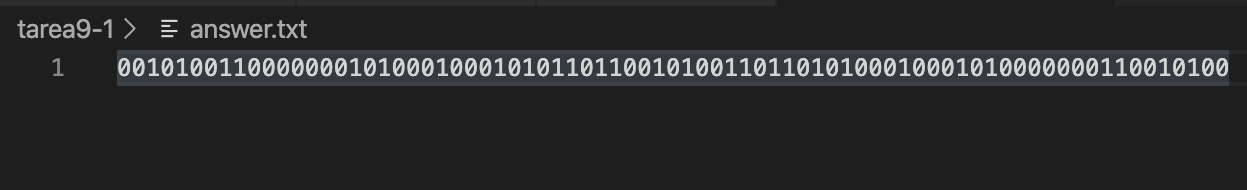
\includegraphics[scale=.60]{tarea9o1}\
	\chapter{S->iCtSA \ A-> eS}
		\section{Programa}
\begin{lstlisting}
#include <stdio.h>
#include <stdlib.h>
/*
if(c){s}s
Compile: gcc app.c
*/
int getBool();
void generateString();
void getString();
int getRandomNumber(int number);

FILE *fanswer;
FILE *fstates;
int length;


int main(int argc, const char **argv)
{
    int n = 100;
    arc4random();
    if (argc == 2)
    {
        n = atoi(argv[1]);
    }
    length = getRandomNumber(n);
    fanswer = fopen("./answer.c", "w");
    fstates = fopen("./states.txt", "w");

    generateString();
    fclose(fanswer);
    fclose(fstates);
}

void generateString()
{
    printf("length: %i\n", length);
    while (length >= 0)
    {
       getString();
    }
    fputc('\n', fanswer);
}

void getString(){
    if (getBool())
    {
        --length;
        fputs("if(/*condition*/)\n{\n", fanswer);
        fputs("S->iCtSA\n", fstates);
        if(getBool())
        {
            getString();
        }
        fputs("\n}\n", fanswer);
        if(getBool())
        {
            fputs("A-> eS\n", fstates);   
            fputs("else\n{\n", fanswer);
            if(getBool()){
                getString();
            }
            fputs("\n}\n", fanswer);
        }
        else{
            fputs("A-> \n", fstates);   
        }
    }
}
int getBool()
{
    return getRandomNumber(2);
}

int getRandomNumber(int number)
{
    int res = rand();
    if (number > 0)
        res = rand() % number;
    return res;
}
\end{lstlisting}
			\subsection{Input}
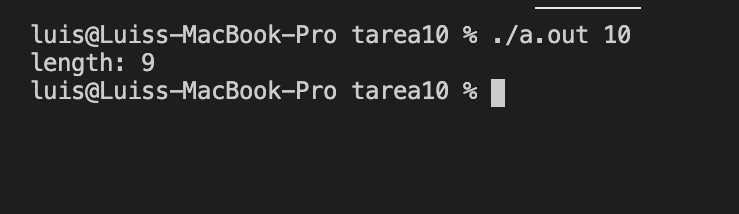
\includegraphics[scale=.60]{tarea10i}\
			\subsection{Output}
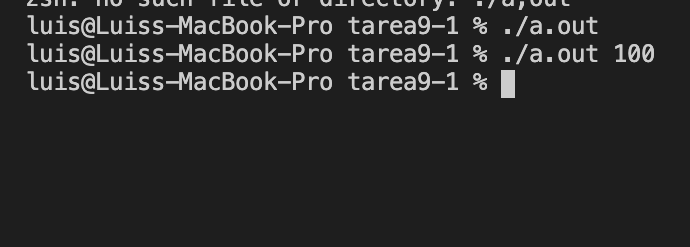
\includegraphics[scale=.60]{tarea9o}\
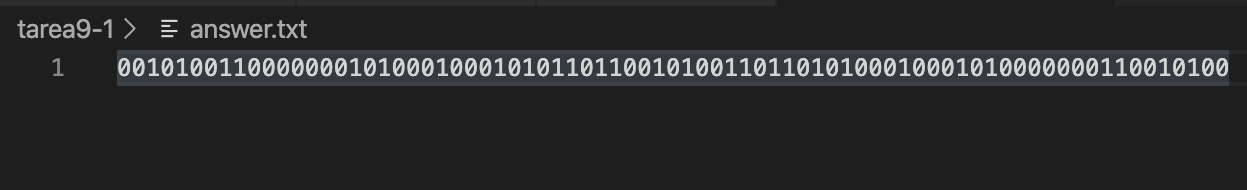
\includegraphics[scale=.60]{tarea9o1}\
	\chapter{Maquina de Turing con Funcionalidad  }
		\section{Programa}
		    \begin{lstlisting}
#include <stdio.h>
#include <stdlib.h>
#include "TADListaDL.h"

/*
Maquina de Turing para 000111
Compile: gcc app.c TADListaDL.c -o a.out
*/

typedef struct container
{
    int to;
    char change;
    int state;
} container;

FILE *fp;
FILE *fanswer;
FILE *fstates;
int aState;

container evaluation(char c, int state);
container evaluation0(int state);
container evaluation1(int state);
container evaluationX(int state);
container evaluationY(int state);
container evaluationB(int state);

boolean validChar(char c);
boolean isValidProcess();

char getChar();

void stateChange(int from, int to);
void generateString();
void generateString(char *, int);
void printContainer(container c);
void printChanges(lista* l);

int getBool();
int getRandomNumber(int number);

int main(int argc, const char **argv)
{
    char *file_name = "./prime.txt";
    if (argc == 2)
    {
        int n = atoi(argv[1]);
        generateString(file_name, n);
    }
    fp = fopen(file_name, "r");
    fstates = fopen("states.txt", "w");
    fanswer = fopen("answer.txt", "w");
    if (isValidProcess())
    {
        printf("Cadena valida\n");
    }
    else
    {
        printf("Cadena no valida\n");
    }
    fclose(fanswer);
    fclose(fstates);
    fclose(fp);
    return 0;
}

boolean isValidProcess()
{
    lista l;
    Initialize(&l);
    container con;
    elemento e;
    posicion p;
    int counter = 0;
    con.state = 0;
    char c = getChar();
    e.c = c;
    Add(&l, e);
    con.to = 1;
    while (con.state != 4 && validChar(c))
    {
        printChanges(&l);
        aState = con.state;
        con = evaluation(c, con.state);
        if (con.state >= 4)
        {
            stateChange(aState, 4);
            break;
        }
        stateChange(aState, con.state);
        e.c = con.change;
        Replace(&l, ElementPosition(&l, counter + 1), e);
        counter += con.to;
        if (con.to == 1)
        {
            if ((Size(&l) - 1) < counter)
            {
                c = getChar();
                if (validChar(c))
                {
                    e.c = c;
                    Add(&l, e);
                }
                else
                {
                    c = 'B';
                }
            }
            else
            {
                p = ElementPosition(&l, counter + 1);
                c = Position(&l, p).c;
            }
        }
        else
        {
            if (Size(&l) < counter)
            {
                c = 'B';
            }
            else
            {
                p = ElementPosition(&l, counter + 1);
                c = Position(&l, p).c;
            }
        }
    }
    if (con.state == 4 && !validChar(getChar()))
    {
        while (!Empty(&l))
        {
            p = First(&l);
            fputc(Position(&l, p).c, fanswer);
            Remove(&l, p);
        }
        Destroy(&l);
        return TRUE;
    }
    Destroy(&l);
    return FALSE;
}

container evaluation(char c, int state)
{
    container res;
    if (c == '0')
    {
        res = evaluation0(state);
    }
    else if (c == '1')
    {
        res = evaluation1(state);
    }
    else if (c == 'X')
    {
        res = evaluationX(state);
    }
    else if (c == 'Y')
    {
        res = evaluationY(state);
    }
    else if (c == 'B')
    {
        res = evaluationB(state);
    }
    return res;
}

container evaluation0(int state)
{
    container res;
    if (state == 0)
    {
        res.change = 'X';
        res.state = 1;
        res.to = 1;
    }
    else if (state == 1)
    {
        res.change = '0';
        res.state = 1;
        res.to = 1;
    }
    else if (state == 2)
    {
        res.change = '0';
        res.state = 2;
        res.to = -1;
    }
    return res;
}

container evaluation1(int state)
{
    container res;
    res.state = 5;
    if (state == 1)
    {
        res.change = 'Y';
        res.state = 2;
        res.to = -1;
    }
    return res;
}

container evaluationX(int state)
{
    container res;
    res.state = 5;
    if (state == 2)
    {
        res.change = 'X';
        res.state = 0;
        res.to = 1;
    }
    return res;
}

container evaluationY(int state)
{
    container res;
    res.change = 'Y';
    res.to = 1;
    if (state == 0)
    {
        res.state = 3;
    }
    else if (state == 1)
    {
        res.state = 1;
    }
    else if (state == 2)
    {
        res.state = 2;
        res.to = -1;
    }
    else if (state == 3)
    {
        res.state = 3;
    }
    return res;
}

container evaluationB(int state)
{
    container res;
    res.state = 5;
    if (state == 3)
    {
        res.change = 'B';
        res.state = 4;
        res.to = 1;
    }
    return res;
}

char getChar()
{
    return (char)fgetc(fp);
}

void generateString(char *fileName, int number)
{
    FILE *generate;
    generate = fopen(fileName, "w");
    int i;
    printf("Generado cadena\n");
    if (number % 2 == 1)
        ++number;
    for (i = 0; i < (number / 2); ++i)
    {
        fputc('0', generate);
    }
    if (number % 2 == 1)
        ++number;
    for (i = 0; i < (number / 2); ++i)
    {
        fputc('1', generate);
    }
    fputc('\n', generate);
    fclose(generate);
}

void printContainer(container c)
{
    printf("\nc: %c\n", c.change);
    printf("state: %d \n", c.state);
    printf("to: %i\n", c.to);
}

boolean validChar(char c)
{
    return (c != '\n' && c != '\t' && c != EOF && c != ' ');
}

void printChanges(lista *l)
{
    int i = 0;
    printf("Cinta \n");
    for(i  = 0; i < Size(l); ++i)
    {
        printf("-------\n");
        printf("---%c---\n", (Position(l,ElementPosition(l, i + 1)).c));
        printf("-------\n");
    }
    printf("-------\n\n");

}

void stateChange(int from, int to)
{
    fprintf(fstates, "q%i -> q%i\n", from, to);
}

int getBool()
{
    return getRandomNumber(2);
}

int getRandomNumber(int number)
{
    int res = rand();
    if (number > 0)
        res = rand() % number;
    return res;
}

	        \end{lstlisting}

			\subsection{Input}
				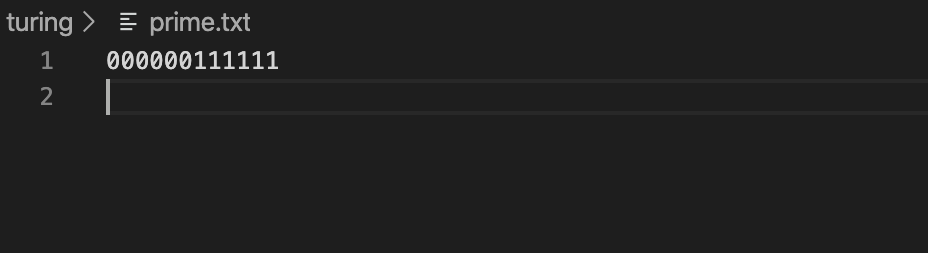
\includegraphics[scale=1.0]{turginI1}\
			\subsection{Output}
				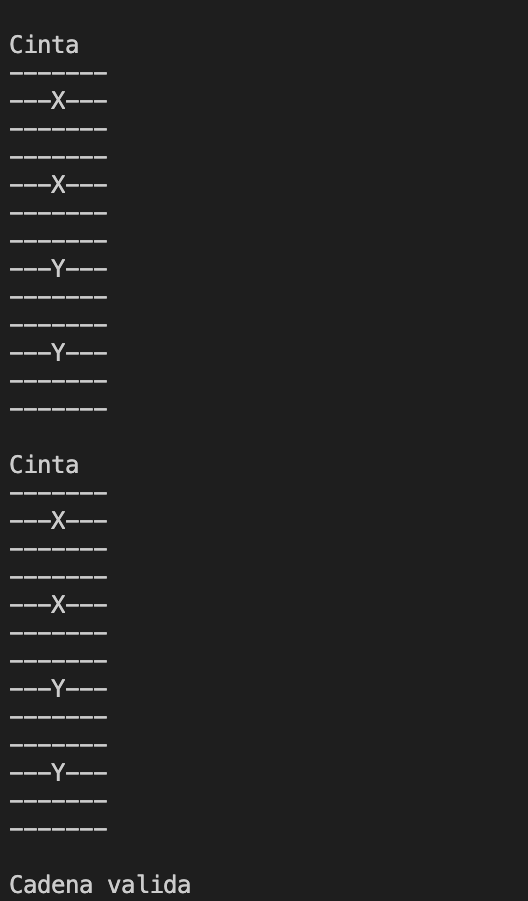
\includegraphics[scale=1.0]{turingO1}\
				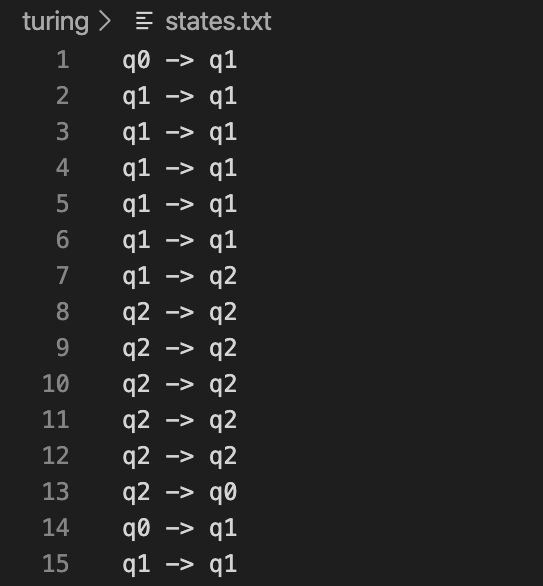
\includegraphics[scale=1.0]{turingO2}
\end{document}